% !TEX root = ../thesis.tex


\chapter{Motivation}
\label{cha:dmd_motivation}
One of the current experiments in our research group probes superfluidity in two-di\-men\-sional Bose gases. In order to achieve a two-dimensional state, the atoms are trapped in a three-dimensional optical box potential which is then compressed in one dimension until one of the motional degrees of freedom is frozen out. 

This trapping geometry is generated from a high powered green laser and another blue-detuned red laser as well as two digital micromirror devices (DMDs) which have the ability to reflect light on a pixel by pixel basis to generate patterns in the intensity distribution. For this trap, one DMD cuts out a rectangle from one beam while the other creates two sheets of light which interfere in the science cell to make a one-dimensional lattice that intersects the rectangular box. The lattice spacing then controls the dimensionality of the system. 
Unfortunately, measurements have shown that the centre of this trap is not completely dark which can be observed through inhomogeneities in the atomic plane. Where these spurious light fields come from is not fully understood, but it is suspected that they stem from reflections of the beams from the science cell.

We want to develop a method to correct for deviations like this using absorption images of the atomic density distribution. A possible setup for this is shown in Figure~\ref{fig:dmd_feedback_sketch}
\begin{figure}[htbp]
    \centering
    % \includegraphics{DMD/FeedbackSketch/FeedbackSketch}
    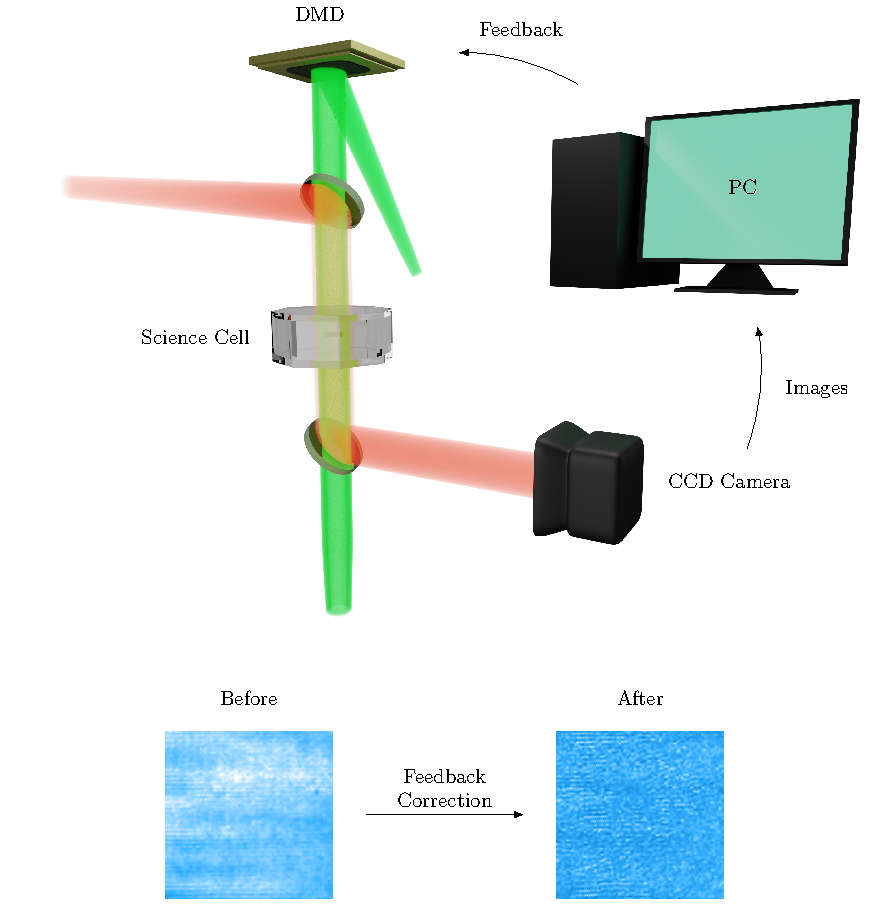
\includegraphics[]{DMD/FeedbackSketch/test1}
    \caption[Proposed setup for adaptive corrections to the DMD pattern]{Proposed setup for adaptive corrections to the DMD pattern. The hollow trapping beam is shown in green, the imaging beam in red.}
    \label{fig:dmd_feedback_sketch}
\end{figure}


In this part, a proof-of-principle correction algorithm is developed using direct imaging of a DMD and a CCD camera.